\subsection{Impact of ESD on electronic devices}

%TODO: Pictures
% Electronic devices are exposed to ESD, in factories first
As detailed in the introduction, electrostatic discharges constitute a large threat for electronic devices.
Failures can occur during manufacturing and or normal operation.
The manipulation of parts by manufacturing machines involves repeated contact and separation.
Ultimately, triboelectrification and discharges happen and devices can get destroyed.
Several standards exist to guarantee that devices can survive this manufacturing step.

% HBM
The Human Body Model (HBM) reproduces the discharge of a human body into a device.
It is standardized in Method 3015.9 of MIL-STD-883 \cite{MIL-STD-883} and JEDEC JS-001-2014 \cite{jedec-001}.
The charged human body is modeled by a 100 pF capacitor and a discharge resistor of 1.5 k\textOmega{}.
Charging voltages reach a maximum of 8kV, although nowadays customers tend to ask for less than that.

% CDM
The Charged Device Model (CDM) is a field-induced ESD test.
The component under test is placed between two charging plates that generate an electric field.
At some point, a grounded pin is brought near any of the pins of the component, forcing the charges to evacuate suddenly.
This test is standardized in \cite{jedec-002}.

% MM
The Machine Model (MM) used to be another ESD testing specification that is now considered deprecated.
The JEDEC committee recommended discontinuing use of this standard \cite{discontinued-mm}, because it is the result of a misunderstanding of real-world events in manufacturing environments.
It does not help improving the reliability of devices against electrostatic discharges.

% HMM ?

%
Over the years, manufacturing processes and standards have improved, reducing the requirements of discharge levels to sustain.
In parallel, the factory environment has been studied extensively to identify actual levels devices are exposed to.
Machine Model deprecation is the perfect illustration of increased community knowledge and experience.
Those efforts aim to reduce the pressure on semiconductor manufacturers that are facing growing challenges to protect devices, because of the shrink of technologies and robustness.

% Electronic devices are exposed to ESD in the field
After manufacturing, failures can happen with the device in the field and exposed to its operating environment.
Manipulation by electrically-charged humans is a major source of danger for commercial products like cellphones and cameras.
The automotive environment is even harsher, with vehicles being a major source of electrostatic discharges.

% Main impact is hard-failure
The electrical destruction of a device is called a hard-failure.
A hard-failure corresponds to changes in the material structure or properties of a device to the point where it no longer fullfills at least part of its specification.
\gls{esd} induce those failures because of the extremely large current densities, high voltages, and power levels involved.
Different kinds of failure signatures can be observed.
Pictures of destroyed devices, obtained with an electronic microscope, are provided in Fig. \ref{fig:silicon-level-failures}.
%TODO: Comment

\begin{figure}[!h]
  \centering
  \includegraphics[width=0.3\textwidth]{src/1/figures/example_silicon_failures.pdf}
  \caption{Example of ESD induced failures at silicon-level}
  \label{fig:silicon-level-failures}
\end{figure}


% Oxyde breakdown
%TODO: Etoffer avec these monnereau
%TODO: Values
A first kind of common failure for integrated devices is the oxyde breakdown.
Oxyde breakdown happens when an insulating material is exposed to a larger electric field than it can tolerate.
During an \gls{esd}, large voltage variations in a short amount of time result in very large electric fields superior to 1kV/m ?
For reference, thunder and lightning events have electrical fields in the same order of magnitude.
Oxyde breakdown is usually discovered in the insulator constituting the gate of a \gls{mos} transistor.
As technologies shrink, so does transistor gate oxyde thickness (TODO: Citer presentation).
A thinner gate oxyde can tolerate less electrical field ?
After the failure, the gate that is normally insulated from the rest of the device leaks significant amount of current.
The transistor can no longer operate and is considered destroyed.

% Thermal breakdown
Thermal breakdown is another kind of ESD induced failure.
It is the result of an elevation of temperature inside the silicon, above its melting point.
It is caused for long discharges that can induce significant and very localized device heating.
It results in a significant increase of leakage current or apparition of short-circuits.

% Metal melt
Finally, metal melt is the last kind of failures observed after a discharge.
Inside an integrated circuit, metal tracks are rather resistive because of their form factor.
Resistivity sits in the range of 10m\textOmega{}/$\Box$ to 100m\textOmega/$\Box$.
When large currents are flowing, metal tracks and vias dissipate power and heat up.
The elevation of temperature, if large enough, can melt the metal track and turn it into an open-circuit.

% Hard-failure is one thing, soft-fail another
Integrated circuits are studied and protected against hard-failure since a few decades.
Despite this experience of the \gls{esd} community, it remains challenging to perfectly protect an electronic system against hard-failures.
Nowadays, a new class of failures appears.
Instead of studying permanent failures, devices are studied for temporary failures affecting their functionality.
These are called soft-failures or functional failures.
\gls{esd} can cause them to happen, with diverse consequences.
In less severe situations, functionnality of a chip is disturbed just for the duration of the ESD and recovers immediately without noticeable consequence.
The failure remains located inside the integrated circuit and does not impact the application above.
Sometimes, the discharge is harmful enough to cause a circuit to restart because the \gls{esd} disturbed some critial nets or parameters.
This is common when supply voltages go out of specification for instance.
Startups or power-on reset functions understands overvoltage or undervoltage as the signal for a regular power-up sequence.
The device can also perform restarts to try a recovery because proper operations cannot be guaranteed, due to unexpected values on some nets.
Most microcontrollers for instance monitor supply voltages of digital gates.
If the voltage is too low, the noise margins of the gates cannot be guaranteed and proper operations either.
At this point, the microcontroller restarts to try to recover.
Restarts are slow processes compared to the operation of a chip.
For critical applications, this delay is highly unwanted because it impacts human safety.
The availability of the chip that triggers airbags in a car is vital for instance.
In a more severe scenario, the system gets completely frozen or stuck into an unwanted state because of the \gls{esd}.
The only way to recover normal operation requires a user-intervention.
User intervention can take the form of turning the key to shut down and restart the vehicle's engine.
Finally, hard-failure can be seen as the next step immediately after the most severe soft-failure.
The device is in a non-recoverable state and must be replaced.
Hard-failures are not considered for functional robustness analysis.

% What is the challenge
In this context, soft-failures represent a risk just as important as hardware failures.
To limit risks and costs inherents to upgrading a device after it was deployed in the field, these failures must be taken care of as early as possible.
Ideally, the robustness of an electronic product should be studied, characterized or simulated during its design phase.
The research conducted and presented in this document aims to develop new tools and techniques for studying and predicting functional failures.

% Protection of integrated circuits against hard-failure is done with ESD protections
To protect sensitive electronics against discharges, several options are available.
The most common solution, presented in the next section, is the \gls{esd} protection.

\subsection{ESD protection}

% Principle of operation
\gls{esd} protections deviate discharge current before it reaches sensitive circuitry and clamp input voltages to avoid crossing the maximum tolerated levels.
Fig. \ref{fig:esd-protection-strategy} gives a simple example of \gls{esd} protection strategy.
Current is routed into the ground before reaching the core-circuitry.
Protections have very low on-resistance, usually in the order of a few ohms.
Even with a few amperes of current, voltage remains low.
\gls{esd} protections can absorb significant amounts of current for very short periods of time, but they are not designed to sustain DC currents.

\begin{figure}[!h]
  \centering
  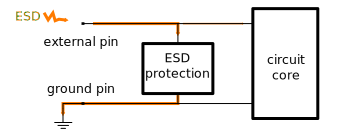
\includegraphics[width=0.3\textwidth]{src/1/figures/esd_protection_strategy.pdf}
  \caption{Classic ESD protection strategy}
  \label{fig:esd-protection-strategy}
\end{figure}

% Types of protection
Inside an electronic circuit, ESD protections are usually found in two different locations.
On-chip protections are integrated directly into silicon.
External protections are discrete devices connected to the input of an \gls{ic}.
Historically, on-chip protections were designed to protect integrated circuits against stresses generated during manufacturing.
They were not aimed to protect against system-level discharges, i.e. discharges happening in the field during the normal product life.
This task was fullfilled by external protections, such as TVS, diodes, capacitors, filters, etc.
Over the years, design techniques and simulations tools improved, and more robust integrated protections could be designed.
On the other hand, equipment manufacturer were always looking for means of reducing the \gls{bom} or the cost of electronic systems.
This lead to a shift of responsabilities for protecting against system-level stresses toward on-chip \gls{esd} protections.
The shrink of integrated technologies makes this tasks ever more challenging.
External protections are still very relevant, where an integration solution would occupy too much silicon area, or when very harsh requirements are demanded.

\begin{figure}[!h]
  \centering
  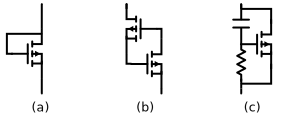
\includegraphics[width=0.3\textwidth]{src/1/figures/architecture_esd_protections.pdf}
  \caption{common ESD protections architectures - (a) Diode (b) Thyristor (c) RC-triggered MOS (d) ?}
  \label{fig:architecture-esd-protection}
\end{figure}

% Implementation and common architectures
ESD protections can be designed in various ways (see Fig. \ref{fig:architecture-esd-protection}).
Diodes are commonly found.
They are not necessarily the more compact solution on silicon, but they can protect properly sensitive circuitry.
Thyristor architectures are frequently used too.
Below triggering voltage, the structure is completely off and disconnected.
Above it, the thyristor switches on, absorbs current, and stays on until the discharges is over and the current returns to a small value.
Thyristors have typical snapback characteristics as shown in Fig. \ref{fig:iv-curve-esd-protection}.
RC-triggered \gls{mos} are frequently found for protecting low-voltage \gls{io} of \gls{cmos} circuits.
Basically, it is a power transistor activated during the discharge by a resistor-capacitor network.
The capacitor is most of the time the parasitic gate capacitance to ground (TODO: check).
During a transient event, the capacitor acts as a short-circuit, rising the gate potential.
The \gls{mos} switches on and absorbs current, deviating it into the ground.

%TODO: Put leakage curve
\begin{figure}[!h]
  \centering
  \includegraphics[width=0.3\textwidth]{src/1/figures/iv_curves_esd_protections.pdf}
  \caption{I(V) curves of typical ESD protections with snapback and no-snapback}
  \label{fig:iv-curve-esd-protection}
\end{figure}

% Comment IV curve
A few key values are important for describing a protection.
V\textsubscript{t1} refers to the triggering voltage of the protection.
I\textsubscript{t1} (snapback devices only ?) corresponds the current absorbed by the protection immediately after triggering.
V\textsubscript{t2} and I\textsubscript{t2} describe the coordinates where the protection is destroyed.
A sudden increase of the leakage current (Fig. \ref{fig:iv-curve-esd-protection}) is a good indicator of a damaged protection.
Leakage current is extracted with a DC source, with a compliancy value set very low, usually below the milli-ampere of current.

%TODO: Talk about protection strategies, centralized clamp vs distributed. RC-mos + boost rail to trigger all protections, etc.

% Requirements
To design a efficient \gls{esd} protection, several constraints and requirements must be fullfilled.
In the absence of a discharge, protections must be transparent to the rest of the device.
The protection must trigger above the operating voltage of the circuitry.
If an input operates between 0V and 5V, and the protection switches on at 4V, it will trigger during normal operation and be immediately destroyed.
On the other hand, protections must trigger below the maximum voltage tolerated by the silicon technology.
If the integrated technology accepts voltages below 50V, and the protection triggers at 60V, the circuit will be destroyed.
Therefore, they are designed to operate between those two boundaries which delimit the \gls{soa} (see Fig. \ref{fig:soa-esd-protection}).
For demanding applications, protections must trigger at a given voltage accurately, independently of manufacturing process, layers mismatches and temperature variation.
This reduces the \gls{soa} substantially and makes the design more challenging.

\begin{figure}[!h]
  \centering
  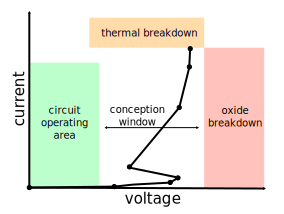
\includegraphics[width=0.3\textwidth]{src/1/figures/esd_protection_soa.pdf}
  \caption{Safe-Operating Area of an ESD protection}
  \label{fig:soa-esd-protection}
\end{figure}

% Tools
To design and validate protections, tools like Centaurus TCAD \cite{TODO} are employed to simulate semiconductor physics.
Afterwards, an electrical model is constructed, to verify that the protection and the circuit cooperate as expected.
Simulation is ran in a \gls{spice} environment, such as Cadence Virtuoso \cite{TODO} or Mentor Graphics SimVision \cite{TODO}.
Modelling of \gls{esd} protections for \gls{spice} simulations is presented later in chapter \ref{esd-protection-modelling}.
